\documentclass[12pt,a4paper]{amsart}

\newcommand{\luigi}[1]{{{\color{red} [Luigi] #1}}}
\newcommand{\gianni}[1]{{{\color{blue} [Gianni] #1}}}

\usepackage[hyphens]{url}
\usepackage[pdftex]{graphicx}
\usepackage{amssymb}
\usepackage{amsthm}
\usepackage{array}
\usepackage{bm}
\usepackage{color}
\usepackage{etex}
\usepackage{extramacros}
\usepackage{fullpage}
\usepackage{graphicx}
\usepackage{hyperref}
\usepackage{mathtools}
\usepackage{stackrel}


\theoremstyle{plain}
\newtheorem{thm}{Theorem}
% \newtheorem{lem}[thm]{Lemma}
\newtheorem{proposition}[thm]{Proposition}
\newtheorem{corollary}[thm]{Corollary}
% \newtheorem*{KL}{Klein’s Lemma}
\newtheorem{definition}[thm]{Definition}

\theoremstyle{definition}
% \newtheorem{conj}{Conjecture}[section]

\theoremstyle{remark}
\newtheorem{example}{Example}
\newtheorem{exercise}{Exercise}
\newtheorem{remark}{Remark}
\newtheorem*{comment}{Comment}
% \newtheorem*{note}{Note}
% \newtheorem{case}{Case}


\begin{document}

\title[Hamming-Wasserstein]{Computing Hamming-Wasserstein distance with the natural gradient flow}

\author[L. Malag\`o]{Luigi Malag\`o}
\address{L. Malag\`o: Romanian Institute of Science and Technology - RIST, Str. Virgil Fulicea nr. 17, 400022 Cluj-Napoca, Romania}
\email{malago@rist.ro}
\urladdr{http://luigimalago.it/}

\author[G. Pistone]{Giovanni Pistone}
\address{G. Pistone: de Castro Statistics, Collegio Carlo Alberto, Piazza Vincenzo Arbarello 8, 10122 Torino, Italy}
\email{giovanni.pistone@carloalberto.org}
\urladdr{https://www.giannidiorestino.it}

\thanks{G. Pistone is supported by the de Castro Statistics Initiative, Collegio Carlo Alberto, Moncalieri; and he is a member of GNAMPA--INdAM} 

\date{\today}

\maketitle

\tableofcontents

\bibliographystyle{amsplain}

\section{Finite State Space: Full Simplex}
\label{sec:1a}
%
Let $\Omega$ be a finite set with $n+1 = \#\Omega$ points. We denote by $\SimO$ the set of the probability functions $p \colon \Omega \to \nonnegreals$, $\sum_{x\in\Omega} p(x) = 1$. It is a $n$-simplex of $\reals^\Omega$ that is, an $n$-dimensional polytope which is the convex hull of its (n + 1) vertexes $\be_x$, $x \in \Omega$. It is a closed and convex convex subset of the affine space $\AffineO = \setof{q \in \reals^\Omega}{\sum_{x\in\Omega} q(x) = 1}$. It has a non empty relative topological interior $\oSimO$, which is the set of the strictly positive probability functions,
%
\begin{equation*}
 \oSimO = \setof{p \in \reals^{\Omega}}{\sum_{x\in\Omega} p(x) = 1, p(x) > 0}.
\end{equation*}
%
The border of the simplex $\SimO$ is the union of all its faces as a convex set. We recall that  a face of maximal dimension $(n-1)$ is called \emph{facet}. Each face is itself a simplex. An \emph{edge} is a face of dimension 1.

\begin{comment}\small
The presentation below does not use explicitly any specific parameterization of the sets $\oSimO$, $\SimO$, $\AffineO$, whose topological and geometrical structure is inherited from $\reals^\Omega$. However, the actual extension of this theory to non finite sample space requires a careful handling as most of the topological features of the finite case do not hold in the infinite case. 

One possibility is given by the so called \emph{exponential manifold}, which were first introduced in \cite{pistone|sempi:95}, and which are Banach manifolds modeled on Orlicz spaces, see the review paper \cite{pistone:2013GSI}. A different option is being developed by the authors of \cite{ay|jost|le|schwachhofer:2015} (private communication), see also \cite{le:2014.1306.1465}. They use as basic topological framework the Banach space of finite signed measures with the total variation norm. Jet another option is to consider the index introduced by Corrado Gini in 1915, now usually called Wasserstein's metric on real probability measures with finite second moments, see e.g. the monograph \cite{ambrosio|gigli|savare:2008}. Other solutions non mentioned here are being studied.  
\end{comment}

\subsection{Statistical bundle}

The idea of this presentation is to consider the probability simplex, that is the set of probability measures, together with the set of integrable functions, to form a vector bundle. Precisely, associated to each probability function $p \in \SimO$ there is a Hilbert space of random variables $L^2(p) = \reals \oplus L^2_0(p)$. We argue that the proper Geometry of Statistics is the geometry of the linear bundle whose elements are $(p,U)$ with $p \in \SimO$ and $U \in L^2_0(p)$. 

\begin{definition}
  The statistical bundle with base $\SimO$ is
%
  \begin{equation*}
    T\SimO = \setof{(p,U)}{p \in \SimO, U \in L^2_0(p)},
  \end{equation*}
%
where $T_p\SimO = L^2_0(p)$ is the space of random variables whose support is contained in the support of $p$ and which are orthogonal to the constant $\one_{\suppof p}$. 
\end{definition}

\begin{comment}\small
This concept variously appears in the literature, cf. \cite{amari:85}, \cite{lauritzen:87ims}, \cite{murray|rice:93}, \cite{gibilisco|pistone:98}, \cite{amari|nagaoka:2000}, \cite{le:2014.1306.1465}.
\end{comment}

The geometry of the statistical bundle $T\SimO$ has a peculiar form of velocity vectors $U \in T_p\SimO$ which are defined in terms of \emph{scores}.

Let $t \mapsto p(t) \in \SimO$ be a curve which is differentiable as a curve in $\reals^\Omega$. Observe that $\scalarof \one {\dot p(t)} = 0$  and call $t \mapsto (p(t),\dot p(t))$ the \emph{velocity curve} which takes values in the trivial bundle $\SimO \times \spanvar{\one}^\perp$. The following is the finite state space version of a result in \cite{2015arXiv151007305A}.

\begin{proposition}
At each $t$ the support of $\dot p(t)$ is contained in the support of $p(t)$, so that $\dot p(t) = Sp(t) \cdot p(t)$, where
%
\begin{equation}\label{eq:score}
Sp(x;t) = 
\begin{cases} 0 & \text{if $p(x;t) = 0$}, \\ \frac{\dot p(x;t)}{p(x;t)} = \derivby t \log p(x;t) & \text{if $p(x;t) > 0$.}
  \end{cases} 
\end{equation}
\end{proposition}

\begin{proof}
For each $t$ and $x \in \Omega$ the condition $p(x;t) = 0$ implies that $t$ is a minimum, hence $\dot p(x;t) = 0$. It follows for all $t$ that $\dot p(t) = Sp(t) \cdot p(t)$.  
\end{proof}

\begin{definition}
The \emph{score} of the differentiable curve $t \mapsto p(t) \in \SimO$ is the curve in the statistical bundle $t \mapsto (p(t),Sp(t)) \in T\SimO$.
\end{definition}

\begin{exercise} \tiny
We first discuss the statistical geometry on the open simplex by deriving it from a \emph{vector bundle} with base $\oSimO$. Later we will show that such a bundle can be identified with the tangent bundle of proper manifold structure. It is nevertheless interesting to observe that a number of geometrical properties do not require the actual definition of the statistical manifold, possibly opening the way to a new type of generalization outside the basic finite state space case.

For each $p \in \oSimO$ we consider the plane through the origin, orthogonal to the vector $\overrightarrow{\text{O}p}$. The set of positive probabilities each one associated to its plane forms a vector bundle which is the basic structure of our presentation of Information Geometry, see Fig.~\ref{fig:tangentbundle}. Note that, because of our orientation to Statistics, we call each element of $\reals^\Omega = L(\Omega)$ a \emph{random variable}. The set of random variables with 0 $p$-expectation is denoted by $L_0(p)$. 
%
% \begin{figure}
% \centering \includegraphics[width=0.30\linewidth, viewport = 67 61 238 233]{Pictures/tangentbundle.pdf}
% \caption{The red triangle is the simplex on the sample space with 3 points $\Omega=\{x,y,z\}$ viewed from below. The blue curve on the simplex is a one-dimensional statistical model. The  probabilities $p$  are represented by vectors from $O$ to the point whose coordinates are $p=(p(x),p(y),p(z))$. The   velocity vectors $Dp(t)$ of a curve $I \mapsto p(t)$ are represented by arrows; they are orthogonal to the vector from $O$ to $p$.\label{fig:tangentbundle}}
% \end{figure}
\end{exercise}

In geometry, a mapping $F$ defined on the  probabilities $p \in \SimO$ to the bundle, compatible with the bundle structure, that is
%
\begin{equation*}
  F \colon p \mapsto (p, F(p)) \in \SimO \times \cup_{p\in\SimO} T_p\SimO) \ ,
\end{equation*}
%
such that $F(p) \in T_p\SimO$---that is, $F(p)$ is a random variable whose support is contained in the support of $p$ and $\expectat p {F(p)} = 0$,--- is called a \emph{section}  of the vector bundle. In Statistics, such a mapping is called an \emph{estimating function} as the equation $F(\hat p,x) = 0$, $x \in \Omega$, provides an \emph{estimator}, that is a distinguished mapping from the sample space $\Omega$ to the simplex of probabilities $\SimO$.
   
We can extend the previous definitions as follows
%
\begin{definition}
\begin{enumerate}
\item Let $\mathcal M$ be a subset of $L^2(\Omega)$. The statistical bundle with base $\mathcal M$ is the linear bundle
%
  \begin{equation*}
    T\mathcal M = \setof{(q,U) \in \mathcal M \times L^2(\Omega)}{\Supp U \subset \Supp p, \sum_{x\in\Omega}  U(x)q(x) = 0} \ .
  \end{equation*}
%
\item Each fiber $T_p\mathcal M$ is endowed with a bilinear form
%
\begin{equation*}
  \scalarat q {U}{V} = \sum_{x\in\Omega} U(x)V(x) \ q(x) \ .
\end{equation*}
\item A continuous curve $t \mapsto q(t) \in \mathcal M \subset L^2(\Omega)$ is S-regular in the statistical bundle if there exists a continuous curve $t \mapsto (p(t),Sq(t)) \in T\mathcal M \subset L^2(\Omega) \times L^(\Omega)$ in the statistical bundle such that for each function $f \colon \SimO \to \reals$ it holds
%
  \begin{equation*}
    \derivby t \sum_{x\in\Omega} f(x) q(x;t) = \scalarat {q(t)} {f - \sum_{x\in\Omega} f(x) q(x;t)}{Sq(t)} \ . 
  \end{equation*}
%
\item A \emph{vector field} $F$ of the statistical bundle is a \emph{section} of the bundles,
%
  \begin{equation*}
    F \colon \mathcal M \ni q \mapsto (q,F(q)) \in T\mathcal M \ . 
  \end{equation*}
%
\end{enumerate}
\end{definition}

\begin{comment}\tiny
The previous definition is suggested by the classical set-up of statistics, as it is revealed by the Fisher-Rao computation. However this set-up is too narrow in a number of situation.
%
\begin{enumerate}
\item The probability functions in the application of interest could have zero values at some $x \in \Omega$, that is the set of interest could be the full simplex $\SimO$. 
\item We shall see soon simple examples where one wants to study a neighborhood of the border of the simplex, namely the full affine space $\AffineO$.
\end{enumerate}

We can give a formal extended definition as follows.
%
\begin{definition}
\begin{enumerate}
\item
For each $\eta \in \AffineO$ let $B_\eta$ be the vector space of random variables $U$ that are $\mu$-centered,
\begin{equation*}
  B_\eta = \setof {U \colon \Omega \to \reals} {\expectat \eta U = \sum_{x\in\Omega} U(x)\ \eta(x) = 0} \ .
\end{equation*}
%
\item
Each $B_\eta$ is endowed with the bi-linear form
%
\begin{equation*}
  \scalarat \eta {U}{V} = \expectat \eta {UV} = \sum_{\setof{x\in\Omega}{\eta(x) \ne 0}} U(x)V(x) \ \eta(x) \ .
\end{equation*}
\item
The \emph{statistical bundle} of the affine space $\AffineO$ is the linear bundle on $\AffineO$
%
\begin{equation*}
  \SAffineO = \setof{(\eta,U)}{\eta \in \AffineO, U \in  B_\eta} \ .
\end{equation*}
%
\item
It is a manifold isomorphic to the open subset of the Grassmanian manifold $\operatorname{Grass}(\reals^\Omega,\#\Omega-1)$ of sub-spaces $B$ that do not contain constant vectors. In fact, each fiber $B_\eta$ is a subspace of $\reals^\Omega$ of co-dimension 1; Viceversa, for each subspace $B$ of dimension $(n-1)$ and not containing the constant, there is a unique complement vector $\eta$ such that $\sum_{x\in\Omega} \eta_x = 1$. 
%
\item A \emph{vector field} $F$ of the statistical bundle of the affine space $\AffineO$ is a \emph{section} of the bundle i.e.,
%
  \begin{equation*}
    F \colon \AffineO \ni \eta \mapsto (\eta,F(\eta)) \in \SAffineO \ . 
  \end{equation*}
%
\end{enumerate}
\end{definition}
\end{comment}

We  now discuss notion of gradient in the statistical bundle.

\begin{proposition}
%
  \begin{enumerate}
  \item Let $I \ni t \mapsto p(t)$ be a $C^1$ curve in $\oSimO$. For each $f \colon \Omega \to \reals$,
%
    \begin{equation*}
      \derivby t \expectat {p(t)} {f} = \scalarat {p(t)} {f -\expectat {p(t)} f} {Dp(t)}, \quad Dp(t) = \derivby t \logof{p(t)} \ .
    \end{equation*}
  \item Let $I \ni t \mapsto \eta(t)$ be a $C^1$ curve in $\AffineO$ such that $\eta(t) \in \SimO$ for all $t$. For all $x \in \Omega$, $\eta(x;t) = 0$ implies $\derivby t \eta(x;t)=0$. Hence, for each $f \colon \SimO \to \reals$,
%
    \begin{equation*}
      \derivby t \expectat {\eta(t)} {f} = \scalarat {\eta(t)} {f - \expectat {\eta(t)} f} {D\eta(t)} \ ,
    \end{equation*}
where
\begin{equation*}
  D\eta(x;t) = \derivby t \log\avalof{\eta(x;t)} \quad \text{if $\eta(x;t) \ne 0$, otherwise 0} .  
\end{equation*}
  \item Let $I \ni t \mapsto \eta(t)$ be a $C^1$ curve in $\AffineO$ and \emph{assume} that  $\eta(x;t) = 0$ implies $\derivby t \eta(x;t)=0$. Hence, for each $f \colon \SimO \to \reals$,
%
    \begin{equation*}
      \derivby t \expectat {\eta(t)} {f} = \scalarat {\eta(t)} {f - \expectat {\eta(t)} f} {D\eta(t)} \ ,
    \end{equation*}
where
\begin{equation*}
  D\eta(x;t) = \derivby t \log\avalof{\eta(x;t)} \quad \text{if $\eta(x;t) \ne 0$, otherwise 0} .  
\end{equation*}
  \end{enumerate}
\end{proposition}

\begin{proof}
  \begin{enumerate}
  \item This part has been already proved in Sec. \ref{sec:Rao}.
  \item Let $x \in \Omega$ and $t \in I$ be such that $\eta(x;t) = 0$. The real function $I \ni s \mapsto \eta(x;s)$ is nonnegative for all $s$ and it is zero at $s=t$. Hence it has a minimum at $s=t$, where the derivative is zero, $0 = \derivby t \eta(x;t) = \dot \eta(x;t)$. As $\dot\eta(x,t) \ne 0$ implies $\eta(x;t) \ne 0$, it holds
%
    \begin{align*}
  \derivby t \expectat {\eta(t)} {f} &= \sum_{x\in\Omega} f(x) \dot\eta(x;t) \\
&= \sum_{\setof{x\in\Omega}{\dot\eta(x,t) \ne 0}} f(x) \ \dot\eta(x;t) \\ 
&= \sum_{\setof{x\in\Omega}{\dot\eta(x,t) \ne 0}} f(x) \ \frac{\dot\eta(x;t)}{\eta(x;t)} \ \eta(x;t) \\ 
&= \sum_{\setof{x\in\Omega}{\eta(x,t) \ne 0}} f(x) \ \frac{\dot\eta(x;t)}{\eta(x;t)} \ \eta(x;t) \\ 
&= \sum_{\setof{x\in\Omega}{\eta(x,t) \ne 0}} f(x) \ \derivby t \log\avalof{\eta(x;t)} \ \eta(x;t) \\ 
&= \scalarat {\eta(t)} {f} {D\eta(t)} \\
&= \scalarat {\eta(t)} {f - \expectat {\eta(t)} f} {D\eta(t)}    
    \end{align*}
  \item Same proof as the second part of the previous item.
  \end{enumerate}
\end{proof}

\begin{definition}[Score]
\begin{enumerate}
\item
If $I \ni t \mapsto p(t) \in \oSimO$ is a $C^1$ curve, its \emph{score} is defined by
%
\begin{equation*}
  D p(t) = \frac{\dot p(t)}{p(t)} = \derivby t \log p(t), \quad t \in I \ .
\end{equation*}
%
As the score $Dp(t)$ is a $p(t)$-centered random variable which belongs to $B_{p(t)}$ for all $t \in I$, the mapping $I \ni t \mapsto (p(t),D p(t))$ is a curve in the statistical bundle.
%
\item
Let $I \ni t \mapsto \eta(t) \in \AffineO$ be a $C^1$ curve and assume that $\eta(x;t) = 0$ implies $\dot\eta(x;t) = 0$. The \emph{score} is defined for $t \in I$ by
%
\begin{equation*}
  Dp(x;t) = \frac{\dot\eta(x;t)}{\eta(x;t)} = \derivby t \log\avalof{\eta(x;t)} \text{if $\mu(x;t) \ne 0$, otherwise 0.}
\end{equation*}
%
As the score $D\eta(t)$ at $t$ is a $\eta(t)$-centered random variable that is, it belongs to $B_{\eta(t)}$ for all $t \in I$, the mapping $I \ni t \mapsto (\eta(t),D\eta(t))$ is a curve in the statistical bundle of $\AffineO$. We say that the curve is \emph{regular}.
%
\end{enumerate}
\end{definition}

\begin{remark}
  The condition for the existence of the score means that the score exists if and only if the curve $t \mapsto \eta(t) \in \AffineO$ hits the faces of $\SimO$ only \emph{tangentially}. For example: $n = 3$, $p(0;t) = t$, $p(1;t) = \sqrt{\frac12 - t^2}$, $p(2;t) = 1 - t - \sqrt{\frac12 - t^2}$. 
\end{remark}

Having defined the score, which is a sort of velocity of the curve, we define the corresponding notion of gradient based on the computation in Sec. \ref{sec:Amari}. As before, we distinguish between the $\SoSimO$ case and the $\SAffineO$ case, even if the first one is a special case of the second one.

\begin{definition}[Statistical gradient]
\begin{enumerate}
\item Given a function $f \colon \oSimO \to \reals$, its \emph{statistical gradient} is a vector field $\oSimO \ni p \mapsto (p,\grad F(p)) \in \SoSimO$ such that for each regular curve $I \ni t \mapsto p(t)$ it holds
  \begin{equation*}
    \derivby t f(p(t)) = \scalarat {p(t)} {\grad f(p(t))} {Dp(t)}, \quad t \in I \ .
  \end{equation*}
%
\item Given a function $f \colon \AffineO \to \reals$, its \emph{statistical gradient} is a vector field $\AffineO \ni \eta \mapsto (\eta,\grad f(\eta)) \in T\AffineO$ such that for each curve $t \mapsto \eta(t)$ with a score $Dp$, it holds
  \begin{equation*}
    \derivby t f(\eta(t)) = \scalarat {\eta(t)} {\grad f(\eta(t))} {D\eta(t)}
  \end{equation*}
\end{enumerate}
\end{definition}

\begin{proposition}[Computing $\grad$]
  \begin{enumerate}
\item
If $f$ is a $C^1$ function on an open subset of $\reals^\Omega$ containing $\oSimO$, by writing $\nabla f(p) \colon \Omega \ni x \mapsto \partiald {p(x)} {f(p)}$, we have the following relation between the statistical gradient and the ordinary gradient:
%
\begin{equation*}
  \grad f (p) = \nabla f(p) - \expectat p {\nabla f(p)} \ .
\end{equation*}
\item
If $f$ is a $C^1$ function on an open subset of $\reals^\Omega$ containing $\AffineO$, we have:
%
\begin{equation*}
  \grad f(\eta) = \nabla f(\eta) - \expectat \eta {\nabla f(\eta)} \ .
\end{equation*}
\end{enumerate}
\end{proposition}


\begin{proof}
In fact,
%
  \begin{multline*}
    \derivby t f(\eta(t)) = \sum_{x\in\Omega} \partiald {p(x)} f(p(x;t) \colon x\in \Omega) \derivby t p(x;t) = \\ \scalarat {\eta(t)} {\grad f(\eta(t))} {Dp(x;t)} = \scalarat {\eta(t)} {\grad f(\eta(t)) - \expectat {\eta(t)} {\grad f(\eta(t))}} {D\eta(t)} = \\  \scalarat {\eta(t)} {\nabla f(\eta(t))} {D\eta(t)} \ ,  
  \end{multline*}
%
where $\grad f(\eta(t)) - \expectat {\eta(t)} {\grad f(\eta(t))}$ is the projection of $\grad f(\eta(t))$ onto $B_{\eta(t)}$ with respect to the scalar product $\scalarat {\eta(t)}{.}{.}$.
\end{proof}

\begin{remark} The Information Geometry on the simplex does not coincide with the geometry of the embedding of the simplex $\oSimO \to \reals^\Omega$, in the sense the statistical bundle is not the tangent bundle of these embedding, see Fig. \ref{fig:tangentbundle}. It will become the tangent bundle of the proper geometric structure which is given by special atlases.
\end{remark}
\begin{remark} We can extend the statistical bundle by taking the linear fibers on $\SimO$ or $\AffineO$. In such cases the bi-linear form $B_\eta \times B_\eta \ni (U,V) \mapsto \expectat \eta {U,V}$ is not always a scalar product. In fact $\scalarat {p} \cdot \cdot$ is not faithful where at least a component of the probability vector is zero, while it is not positive definite outside the simplex $\SimO$.
\end{remark}

\begin{remark}
The vector $D p(t) \in B_{p(t)}$ is meant to represent the relative variation of the information in a one dimensional statistical model in the sense it is a relative derivative. Geometrically, the score is a representation of the velocity along a curve, because of the geometric interpretation of C. R. Rao's already mentioned classical computation of Sec.~\ref{sec:Rao}.
\end{remark}

\begin{remark} \label{rem:gradient-tangent}
Consider the level surface of $f \colon \AffineO \to \reals$ at $\eta_0 \in \AffineO$, that is the surface $\setof{\eta \in \AffineO}{f(\eta) = f(\eta_0)}$, and assume $\eta_0$ is not a critical point, $\grad f(\eta_0) \ne 0$. Then for each curve through $\eta_0$, $I \mapsto \eta(t)$ with $\eta(0) = \eta_0$, such that $f(\eta(t)) = f(\eta(0))$, we have
%
\begin{equation*}
  0 = \left. \derivby t f(\eta(t)) \right|_{t=0} = \left. \scalarat {\eta(t)} {\grad f(p(t))} {Dp(t)} \right|_{t=0} = \scalarat {\eta_0} {\nabla f(\eta_0)} {D\eta(t_0)} \ ,
\end{equation*}
%
that is, \emph{all velocities $Dp(t_0)$ tangential to the level set are orthogonal to the statistical gradient}. Note that we have not jet defined a manifold such that the statistical bundle is equal to the tangent bundle. 
\end{remark}

\begin{remark}
If the function $f \colon \AffineO \to \reals$ extends to a $C^1$ function on an open subset of $\reals^\Omega$, then we can compute the statistical gradient via the ordinary gradient in the geometry of $\reals^\Omega$, namely $\nabla f(\eta) \colon \Omega \ni x \mapsto \partiald {\eta(x)} {f(\eta)}$.  Note that the statistical gradient is zero if, and only if, the ordinary gradient is constant.
\end{remark}

\begin{definition}[Flow]
\begin{enumerate}
\item Given a vector field $F \colon \oSimO$ or $F \colon \AffineO$, the \emph{trajectories along the vector field} are the solution of the (statistical) \emph{differential equation}
%
  \begin{equation*}
    \Derivby t p(t) = F(p(t)) \ .
  \end{equation*}
%
In the case $F \colon \oSimO$, the statistical differential equation is equivalent to the ordinary differential equation
%
\begin{equation*}
  \derivby t p(t) = p(t)F(p(t)) \ .
\end{equation*}
\item A \emph{flow} of the vector field $F$ is a mapping $S \colon \oSimO \times \posreals \ni (p,t) \mapsto S(p,t) \in \oSimO$, respectively $S \colon \AffineO \times \posreals \ni (p,t) \mapsto S(p,t) \in \AffineO$, such that $S(p,0) = p$ and $t \mapsto S(p,t)$ is a trajectory along $F$.
\item
Given $f \colon \oSimO \to \reals$, or $f \colon \AffineO \to \reals$, with statistical gradient $p \mapsto (p,\grad f(p)) \in \SoSimO$, respectively $\eta \mapsto (\eta,\grad f(p)) \in \SAffineO$, a solution of the \emph{statistical gradient flow equation}, starting at $p_0 \in \oSimO$, respectively $\eta_0 \in \AffineO$, at time $t_0$, is a trajectory of the field $- \grad f$ starting at $p_0$, respectively $\eta_0$.
\item
The \emph{gradient flow} is the flow of the vector field $- \grad f$.
\end{enumerate}
\end{definition}

\begin{proposition}
\begin{enumerate}
\item
  If $\reals_+ \ni t \mapsto p(t)$ is a solution of the gradient flow of a bounded $f \colon \oSimO \to \reals$, namely, $Dp(t) = -\grad f(p(t))$, $t > 0$, then $t \mapsto f(p(t))$ is decreasing and bounded below by $- \min f$ . 
\item If moreover $t \mapsto \normat {p(t)} {\grad f(p(t))} ^2 = \normat {p(t)} {Dp(t)} ^2$ is uniformly continuous, then $\lim_{t \to \infty} \normat {p(t)} {Dp(t)} = 0$. 
\item Assume in addition that $p \mapsto \normat p {\grad f(p)}$ continuously extend to $L \colon \SimO$ and there exists a level set $\setof{p \in \oSimO}{L(p) \le a}$ where $L$ has an unique zero $\bar p \in \SimO$. Hence, $f(p(0)) \le \alpha$ implies $\lim_{t\to\infty} p(t) = \bar p$.
\end{enumerate}
\end{proposition}

\begin{proof}
\begin{enumerate}
\item   If $p(\cdot)$ is a solution of the statistical gradient flow $Dp(t) = - \grad f(p(t))$, $t > 0$, then 
%
  \begin{equation*}
    \derivby t f(p(t)) = \scalarat {p(t)} {- \grad f(p(t))} {Dp(t)} = - \normat {p(t)} {\grad f(p(t))} ^2 = - \normat {p(t)} {Dp(t)} ^2 \ .
  \end{equation*}
%
It follows that 
%
\begin{equation*}
  f(p(t)) - f(p(0)) =  - \int_0^t \normat {p(t)} {\grad f(p(t))} ^2 \ dt = - \int_0^t \normat {p(t)} {Dp(t)} ^2 \ dt \ ,
\end{equation*}
%
so that $t \mapsto f(p(t))$ is decreasing and converging to a limit $\alpha \ge \min f$. 
\item It follows from the boundedness below of $f$ that $\alpha$ if finite and moreover
%
\begin{equation*}
 \int_0^\infty \normat {p(t)} {\grad f(p(t))} ^2 \ dt =  \int_0^t \normat {p(t)} {Dp(t)} ^2 \ dt \le - \min f < \infty \ .
\end{equation*}
%
As we have assumed that $t \mapsto \normat {p(t)} {\grad f(p(t))} ^2 = \normat {p(t)} {Dp(t)} ^2$ is uniformly continuous, it follows from Barbalat's lemma that $\lim_{t \to \infty} \normat {p(t)} {\grad f(p(t))} = \lim_{t \to \infty} \normat {p(t)} {Dp(t)} = 0$. 
\item It follows that $\lim_{t \to \infty} \normat {p(t)} {\grad f(p(t))} = \lim_{t \to \infty} L(p(t)) = 0$. Every solution that starts inside $\set{f \le a}$ stays in the level set. If $p \mapsto L(p)$ has a unique isolated zero at $\bar p$, then $\lim_{t\to\infty} p(t) = \bar p$.
\end{enumerate}
\end{proof}

\begin{example}[Expected value]
  Let $f \colon \Omega \to \reals$ have a unique maximum at $\bar x$ and relax $f(\eta) = \expectat \eta f$, $\eta \in \AffineO$. We have $\grad f(\eta) = f - \expectat \eta f$. The function $f \colon \SimO$ is bounded and $p \mapsto \normat p {\grad f}^2 = \varat p f$ is bounded and continuous on $\SimO$. The trajectory is the exponential family $p(t) = \euler^{tf - \psi(t)} p_0$ and $Dp(t) = f - \psi'(t)$ is uniformly continuous because its derivative $\derivby t Dp(t) = - \psi''(t) = \varat {p(t)} f$ is bounded.
\end{example}

\section{Finite State Space: Connections}
\label{sec:finite-state-space-connections}

We are now going to discuss now the notion of of differentiable function on the statistical bundle which is a sort of second order calculus, given the relation of the fibers of the statistical bundle with the tangent bundle. Cf. \cite{kass|vos:1997}. 

\subsection{Transports}
\label{sec:transports}
%
 
For each random variable $U \in B_p$, it holds $\expectat q {U - \expectat q U} = 0$ and $\expectat q{\frac pq U} = 0$, so that both $U - \expectat q U$ and $\frac pq U$ belong to $B_q$. 
%
\begin{definition} [e- and m-transport]
\label{def:transport-em}
  \begin{enumerate}
  \item The \emph{exponential transport}, or \emph{e-transport}, is the family of linear mappings
    \begin{equation*}
      \etransport p q \colon B_p \ni U \mapsto U - \expectat q U \in B_q \ .
    \end{equation*}
  \item The \emph{mixture transport}, or \emph{m-transport}, is the family of linear mappings
    \begin{equation*}
      \mtransport p q \colon B_p \ni U \mapsto \frac p q U \in B_q \ .
    \end{equation*}
  \end{enumerate}
\end{definition}

\begin{proposition} \ 
  \begin{enumerate}
  \item Exponential semi-group property: $\etransport q r \etransport p q = \etransport p r$.
  \item Mixture semi-group property: $\mtransport q r \mtransport p q = \mtransport p r$.
  \item Duality: $\scalarat q {\etransport p q U} {V} = \scalarat p {U} {\mtransport q p V}$.
  \item Conservation of the scalar product: $\scalarat q {\etransport p q U}{\mtransport p q V} = \scalarat p U V$.
  \end{enumerate}
  \end{proposition}
%
  \begin{proof}
Simple checks of the definitions.    
  \end{proof}

Each transport defines a vector field of the statistical bundle: given $U \in B_p$, we have the vector fields
%
\begin{equation*}
  q \mapsto \etransport p q U, \quad q \mapsto \mtransport p q U \ ,
\end{equation*}
%
%
and we can compute their respective flows. 

%
\begin{proposition}
  \begin{enumerate}
  \item The flow of the vector field $p \mapsto \etransport q p U$, $U \in \ B_q$ i.e., the solution of 
%
    \begin{equation*}
      Dp(t) = \etransport q {p(t)} U, \quad p(0) = p,
    \end{equation*}
%
 is 
%
 \begin{equation*}
  \oSimO \times \reals \ni (p,t) \mapsto \euler^{t(\etransport q p U) - \psi(t)} \cdot p \ ,
 \end{equation*}
%
where $\quad \psi(t) = \logof{\expectat p {\euler^{\etransport q p U}}}$.
%
\item The flow of the vector field $p \mapsto \mtransport q p U$, $U \in \ B_q$ i.e., the solution of 
%
    \begin{equation*}
      Dp(t) = \mtransport q {p(t)} U, \quad p(0) = p,
    \end{equation*}
%
 is 
%
 \begin{equation*}
  \oSimO \times I \ni (p,t) \mapsto (1+t\mtransport q p U)p \ ,
 \end{equation*}
%
where $I = ]a,b[$, $a = - (\max \mtransport q p U)^{-1}$, $b = - (\min \mtransport q p U)^{-1}$.
\end{enumerate}
\end{proposition}

\begin{proof}
  \begin{enumerate}
  \item Direct check:
%
    \begin{equation*}
      \derivby t (t\etransport q p U - \psi(t))  = \etransport q p U - \dot \psi(t) = \etransport q p U - \expectat {p(t)} {\etransport q p U} = \etransport p {p(t)} \etransport q p U =  \etransport q {p(t)} U \ . 
    \end{equation*}
%
  \item Assume $U \ne 0$ and let $V(x) = \mtransport q p U(x)$. As $\expectat p V = 0$, we can have both $V(x) < 0$ and $V(x) > 0$. In the first case, $1 + tV(x) > 0$ if $t \le 0$ or $t>0$ and $t < -(min V)^{-1} \le -V(x)^{-1}$. Similarly in the other case. With $t \in I$ we have $p(t) = (1+tV)p \in \oSimO$ and
%
    \begin{equation*}
      \derivby t \logof{(1+t\mtransport q p)p} = \frac{\mtransport q p U}{1+t\mtransport q p U} = \frac p {p(t)} \mtransport q p U = \mtransport {p(t)} p \mtransport q p U = \mtransport q {p(t)} U \ .
    \end{equation*}
  \end{enumerate}
\end{proof}

The proposition, in turn, explains the name given to the transports.

Other transports are of interest. In particular we look for an isometry from $B_p$ to $B_q$. Note that $\normat q {\sqrt{\frac pq} U}^2 = \normat p U$ for $U \in B_p$, but $\expectat q {\sqrt{\frac pq} U} = \expectat p {\sqrt{pq} U} = \covat p {\sqrt{pq}}{U}$ is not zero in general. We look for a mapping of the form $B_p \ni U \mapsto \sqrt{\frac pq} U + A\expectat q {\sqrt{\frac pq} U}$. The expected value at $q$ is
%
\begin{equation*}
  \expectat q {\sqrt{\frac pq} U + A\expectat q {\sqrt{\frac pq} U}} = \left(1+\expectat q A\right)\expectat q {\sqrt{\frac pq} U} \ ,
\end{equation*}
%
which is zero if $\expectat q A = -1$. Under this condition we have $\sqrt{\frac pq} U + A\expectat q {\sqrt{\frac pq} U} \in B_q$. Let us compute the squared norm:
%
\begin{multline*}
  \normat q {\sqrt{\frac pq} U + A\expectat q {\sqrt{\frac pq} U}}^2 = \\ \normat p U ^2 + 2\expectat q {\sqrt{\frac pq} U A} \expectat q {\sqrt{\frac pq} U} + \expectat q {A^2} \expectat q {\sqrt{\frac pq} U}^2 = \\ \normat p U ^2 + \left(2\expectat q {\sqrt{\frac pq} U A}  + \expectat q {A^2} \expectat q {\sqrt{\frac pq} U} \right) \expectat q {\sqrt{\frac pq} U} = \\ \normat p U ^2 + \expectat q {\sqrt{\frac pq} U \left(2A + \expectat q {A^2} \right) } \expectat q {\sqrt{\frac pq} U} \ .
\end{multline*}

If we take $ A = - \left(1+\sqrt{\frac pq}\right)/\left(1 + \expectat q {\sqrt{\frac pq}}\right)$ we have both $\expectat q A = -1$ and
%
\begin{multline*}
  \expectat q {\sqrt{\frac pq} U \left(2A + \expectat q {A^2} \right) } = \\
 \expectat q {\sqrt{\frac pq} U \left(-2\frac{1+\sqrt{\frac pq}}{1 + \expectat q {\sqrt{\frac pq}}} + \frac{\expectat q {\left(1+ \sqrt{\frac pq}\right)^2}}{\left(1+\expectat q {\sqrt{\frac pq}}\right)^2} \right) } = \\ \expectat q {\sqrt{\frac pq} U \left(-2\frac{1+\sqrt{\frac pq}}{1 + \expectat q {\sqrt{\frac pq}}} + 2 \frac{1+ \expectat q {\sqrt{\frac pq}}}{\left(1+\expectat q {\sqrt{\frac pq}}\right)^2} \right) } = \\ \expectat q {\sqrt{\frac pq} U \left(-2\frac{1+\sqrt{\frac pq}}{1 + \expectat q {\sqrt{\frac pq}}} + 2 \frac{1}{1+\expectat q {\sqrt{\frac pq}}} \right) } = \\ -2 \frac{\expectat q {\sqrt{\frac pq} U \sqrt{\frac pq} }}{1+\expectat q {\sqrt{\frac pq}}} = 0 \ .
\end{multline*}

The previous computation justifies the following definition and proposition.

\begin{definition}
The \emph{Hilbert transport}, or \emph{h-transport}, is the family of linear mappings
%
    \begin{equation*}
  \htransport p q \colon B_p \ni U \mapsto \sqrt{\frac pq} U  -  \left(1 +  \expectat q {\sqrt{\frac pq}}\right)^{-1} \left(1 + \sqrt{\frac pq}\right) \expectat q {\sqrt{\frac pq}U} \in B_q
    \end{equation*}
\end{definition}

\begin{proposition}
  \begin{enumerate}
  \item Inverse: $\htransport q p \htransport p q u = u$.
  \item Isometry: $\scalarat q {\htransport p q U}{\htransport p q V} = \scalarat p U V$.
  \end{enumerate}
  \end{proposition}
%
  \begin{proof}
    \begin{enumerate}
    \item It is a long computation. Let $V = \htransport p q U$, so that
 %
     \begin{multline*}
\sqrt \frac qp V = 
\sqrt{\frac qp}\left(\sqrt{\frac pq} U  -  \left(1 +  \expectat q {\sqrt{\frac pq}}\right)^{-1} \left(1 + \sqrt{\frac pq}\right) \expectat q {\sqrt{\frac pq}U}\right) = \\ U  -  \left(1 +  \expectat q {\sqrt{\frac pq}}\right)^{-1} \left(1 + \sqrt{\frac qp}\right) \expectat q {\sqrt{\frac pq}U} \ ,
      \end{multline*}
%
      \begin{multline*}
 \expectat p {\sqrt \frac qp V} = \expectat p {U  -  \left(1 +  \expectat q {\sqrt{\frac pq}}\right)^{-1} \left(1 + \sqrt{\frac qp}\right) \expectat q {\sqrt{\frac pq}U}} = \\ -  \left(1 +  \expectat q {\sqrt{\frac pq}}\right)^{-1} \expectat p {1 + \sqrt{\frac qp}} \expectat q {\sqrt{\frac pq}U} = \\ -  \left(1 +  \expectat q {\sqrt{\frac pq}}\right)^{-1} \left(1 + \expectat p {\sqrt{\frac qp}}\right) \expectat q {\sqrt{\frac pq}U} \ ,
      \end{multline*}
%
      \begin{multline*}
\left(1+\expectat p {\sqrt\frac qp}\right)^{-1} \left(1+ \sqrt\frac qp \right) \expectat p {\sqrt \frac qp V} = \\
- \left(1+\expectat p {\sqrt\frac qp}\right)^{-1} \left(1+ \sqrt\frac qp \right) \left(1 +  \expectat q {\sqrt{\frac pq}}\right)^{-1} \left(1 + \expectat p {\sqrt{\frac qp}}\right) \expectat q {\sqrt{\frac pq}U} = \\
-  \left(1+ \sqrt\frac qp \right) \left(1 +  \expectat q {\sqrt{\frac pq}}\right)^{-1} \expectat q {\sqrt{\frac pq}U} \ ,
      \end{multline*}
%
and the required equality follows.
    \item The conservation of the norm is proved above. The conservation of the scalar product follows from that and from the linearity.
    \end{enumerate}
  \end{proof}

  \begin{proposition}
    Given $p \in \oSimO$ and $U \in B_p$ with $\expectat p {U^2} = 1$, consider the mapping on an open interval $I$ containing 0 defined by 
%
    \begin{equation*}
      I \ni t \mapsto \left(\cosof{\frac t2}+\sinof{\frac t2} U\right)^2 \cdot p \ ,
    \end{equation*}
with $\cosof{\frac t2}+\sinof{\frac t2} U >$ for all $t \in I$. Such a mapping is a regular curve in $\oSimO$ such that $p(0) = 0$ and $Dp(t) = \htransport p {p(t)} U$.
  \end{proposition}
%
  \begin{proof}
    First, we check
%
    \begin{multline*}
      \expectat p {\left(\cosof{\frac t2}+\sinof{\frac t2} U\right)^2} = \\ \cossqof{\frac t2} + 2 \cosof{\frac t2} \sinof{\frac t2} \expectat p {U} + \sinsqof{\frac t2} \expectat p {U^2} = 1 \ . 
    \end{multline*}

Second, we compute the score:
%
\begin{multline*}
  Dp(t) = \derivby t 2 \logof{\cosof{\frac t2}+\sinof{\frac t2} U} = \\
2 \frac{-\frac12 \sinof{\frac t2} + \frac12 \cosof{\frac t2}U}{\cosof{\frac t2}+\sinof{\frac t2} U} = \frac{- \sinof{\frac t2} + \cosof{\frac t2}U}{\cosof{\frac t2}+\sinof{\frac t2} U} \ .
\end{multline*}

Third, we compute $\htransport p {p(t)} U$ in steps:
%
\begin{equation*}
  \sqrt{\frac{p}{p(t)}} = \frac1{\cosof{\frac t2}+\sinof{\frac t2} U} \ ;
\end{equation*}
%
\begin{equation*}
  \expectat {p(t)} {\sqrt{\frac{p}{p(t)}}} =  \expectat {p} {\sqrt{\frac{p(t)}{p}}} = \expectat p {\cosof{\frac t2}+\sinof{\frac t2} U} = \cosof{\frac t2} \ ; 
\end{equation*}
%
\begin{multline*}
  \frac{1+\sqrt{\frac{p}{p(t)}}}{1+\expectat {p(t)} {\sqrt{\frac{p}{p(t)}}}} = \left(1+\frac1{\cosof{\frac t2}+\sinof{\frac t2} U}\right) \frac1{1+\cosof{\frac t2}} = \\ \frac{1+\cosof{\frac t2}+\sinof{\frac t2} U}{\cosof{\frac t2}+\sinof{\frac t2} U} \frac1{1+\cosof{\frac t2}} \ ;
\end{multline*}
%
\begin{equation*}
  \sqrt{\frac{p}{p(t)}}U = \frac{U}{\cosof{\frac t2}+\sinof{\frac t2} U} \ ;
\end{equation*}
%
\begin{equation*}
  \expectat {p(t)} {\sqrt{\frac{p}{p(t)}}U} =   \expectat {p} {\sqrt{\frac{p(t)}{p}}U} = \expectat p {\left(\cosof{\frac t2}+\sinof{\frac t2} U\right)U} = \sinof{\frac t2} \ ;
\end{equation*}
%
\begin{multline*}
  \htransport p {p(t)} U =
  \frac{U}{\cosof{\frac t2}+\sinof{\frac t2} U} - \frac{1+\cosof{\frac t2}+\sinof{\frac t2} U}{\cosof{\frac t2}+\sinof{\frac t2} U} \frac{\sinof{\frac t2}}{1+\cosof{\frac t2}} = \\ \frac{\left(1+\cosof{\frac t2}\right)U - \left(\sinof{\frac t2} + \sinof{\frac t2}\cosof{\frac t2}+\sinsqof{\frac t2} U\right)}{\left(\cosof{\frac t2}+\sinof{\frac t2} U\right)\left(1+\cosof{\frac t2}\right)} = \\ \frac{\left(1+\cosof{\frac t2} - \sinsqof{\frac t2}\right)U - \left(\sinof{\frac t2} + \sinof{\frac t2}\cosof{\frac t2} \right)}{\left(\cosof{\frac t2}+\sinof{\frac t2} U\right)\left(1+\cosof{\frac t2}\right)} = \\ \frac{\cosof{\frac t2}U - \sinof{\frac t2}}{\cosof{\frac t2}+\sinof{\frac t2} U} \ . 
\end{multline*}
  \end{proof}

\subsection{Connections}
\label{sec:connections}

Second order geometry is usually based on a notion of covariant derivative or a notion of connection. It leads to interesting applications in optimization, such as the use of a Newton method based on the computation of the proper Hessian. Here we restrict to a definition of acceleration based on the use of transports.

Let us compute the acceleration of a curve $I \mapsto p(t)$. The velocity is $t \mapsto (p(t),Dp(t)) = \left(p(t), \derivby t \logof {p(t)} \right) \in \ToSimO$. The vector $Dp(t)$ has to be checked against an element of $B_{p(t)}$, say $\mtransport p {p(t)} v$. We can compute an acceleration as
%
\begin{align*}
  \derivby t \scalarat {p(t)} {Dp(t)}{\mtransport p {p(t)} v} &= \derivby t \scalarat {p} {\etransport {p(t)} p Dp(t)}{v} \\ &= \scalarat {p} {\derivby t \etransport {p(t)} p Dp(t)}{v} \\ &=  \scalarat {p(t)} {\etransport p {p(t)} \derivby t \etransport {p(t)} p Dp(t)}{\mtransport p {p(t)} v}  
\end{align*}

The \emph{exponential acceleration} is
%
\begin{align*}
  \eacc p(t) &= \etransport p {p(t)} \derivby t \etransport {p(t)} p Dp(t) \\ &=  \etransport p {p(t)} \derivby t \left(\frac{\dot p(t)}{p(t)} - \expectat p {\frac{\dot p(t)}{p(t)}}\right) \\ &=  \etransport p {p(t)} \left(\frac{\ddot p(t)p(t)-\dot p(t)^2}{p(t)^2} - \expectat p {\frac{\ddot p(t)p(t)-\dot p(t)^2}{p(t)^2}}\right) \\ &= \frac{\ddot p(t)p(t)-\dot p(t)^2}{p(t)^2} - \expectat {p(t)} {\frac{\ddot p(t)p(t)-\dot p(t)^2}{p(t)^2}} \\ &= \frac{\ddot p(t)}{p(t)} - (Dp(t))^2 + \expectat {p(t)} {(Dp(t))^2} \ .
\end{align*}

\emph{Exponential families have null exponential acceleration}. In fact for $p(t) = \expof{tU - \psi(t)} p$, we have $\etransport {p(t)} p Dp(t) = U - \expectat p U$, so that $\derivby t \etransport {p(t)} p Dp(t) = 0$. Moreover, note that
%
\begin{align*}
  (Dp(t))^2 &= (u - \dot \psi(t))^2 \ ,\\
  \ddot p(t) &= \derivby t [p(t)(u - \dot \psi(t))] = p(t)(u-\dot\psi(t))^2 - p(t)\ddot\psi(t) \ . 
\end{align*}

A second option is to compute the acceleration as
%
\begin{align*}
  \derivby t \scalarat {p(t)} {Dp(t)}{\etransport p {p(t)} v} &= \derivby t \scalarat {p} {\mtransport {p(t)} p Dp(t)}{v} \\ &= \scalarat {p} {\derivby t \mtransport {p(t)} p Dp(t)}{v} \\ &=  \scalarat {p(t)} {\mtransport p {p(t)} \derivby t \mtransport {p(t)} p Dp(t)}{\etransport p {p(t)} v} \ , 
\end{align*}
%
hence we can compute the \emph{mixture acceleration} as follows
%
\begin{align*}
 \macc p(t) &= \\  \mtransport p {p(t)} \derivby t \mtransport {p(t)} p Dp(t) &=  \frac {p}{p(t)} \derivby t \left(\frac {p(t)}{p} \frac {\dot p(t)}{p(t)}\right) \\ &= \frac {\ddot p(t)}{p(t)} \ . 
\end{align*}

In follows that \emph{mixture models $t \mapsto (1+tU)p$ have null mixture acceleration}.

We could compute the \emph{Riemannian acceleration} as $\htransport p {p(t)} \derivby t \htransport {p(t)} p Dp(t)$. See some developments in \cite{pistone:2013Entropy,pistone:2013GSI,lods|pistone:2015}.

Let us compute the Taylor formula. Given a regular function $f \colon \oSimO \to \reals$ and a regular curve $t \mapsto p(t)$, the first and second derivatives of $t \mapsto f(t)$ are:
%
\begin{align*}
  \derivby t f(p()) &= \scalarat {p(t)} {\grad f(p(t))}{Dp(t)} \\
&= \scalarat {p} {\mtransport {p(t)} p \grad f(p(t))}{\etransport {p(t} p Dp(t)} \ ; 
\end{align*}
%
\begin{align*}
  \dderivby t f(p(t)) &= \scalarat {p} {\derivby t \mtransport {p(t)} p \grad f(p(t))}{\etransport {p(t} p Dp(t)} \\ &\phantom{=}+
\scalarat {p} {\mtransport {p(t)} p \grad f(p(t))}{\derivby t \etransport {p(t} p Dp(t)} \\
&= \scalarat {p(t)} {\mtransport p {p(t)} \derivby t \mtransport {p(t)} p \grad f(p(t))}{Dp(t)} \\ &\phantom{=}+
\scalarat {p(t)} {\grad f(p(t))}{\eacc p(t)} \\ .
\end{align*}

Assume now that $p(t) = \euler^{tU-\psi(t)} p$, $U \in B_p$, so that $\eacc p(t) = 0$, and define the \emph{mixture Hessian} (m-Hessian) to be
%
\begin{equation*}
  \mhessianat U {f(p)} = \left. \mtransport p {p(t)} \derivby t \mtransport {p(t)} p \grad f(p(t)) \right|_{t=0} \in B_p \ . 
\end{equation*}
%
In such a case the second derivative above reduces to
%
\begin{equation*}
    \dderivby t f(p(t)) = \scalarat {p(t)} {\mhessianat {Dp(t)} {f(p(t))}} {Dp(t)} = \scalarat {p(t)} {\mhessianat {U - \dot\psi(t)} {f(p(t))}} {U - \dot\psi(t)}
\end{equation*}
%
and we can write for $q = \euler^{U-\psi(1)}p$,
%
\begin{align*}
  f(q) - f(p) &= \scalarat p {\grad f(p)}{U} + \int_0^1 (1-t) \scalarat {p(t)} {\mhessianat {U - \dot\psi(t)} {f(p(t))}} {U - \dot\psi(t)} \ dt \\
&= \scalarat p {\grad f(p)}{U} + \frac12 \scalarat {p} {\mhessianat {U} {f(p)}} {U} + R_2(p,U) \ .
\end{align*}

In a similar way we could derive a Taylor formula for the e-Hessian and the usual Riemannian Taylor formula as in \cite{absil|mahony|sepulchre:2008}.

\subsection{Atlases}
\label{sec:exponentialatlas}

We have shown in the previous sections how to derive a calculus on the statistical bundle. We now turn to the explicit introduction of special atlases of charts on the statistical bundle. Each of atlas will have the following special properties:
%
\begin{itemize}
\item The tangent space computed in the atlas is the corresponding fiber of the statistical bundle;
\item The tangent space of the bundle induces one of the connections.
\end{itemize}

\begin{definition}[Exponential atlas]
For each $p \in \oSimO$ we define
\begin{equation*}
s_p \colon \SoSimO \ni (q,w) \mapsto \left(\log\frac q p - \expectat p {\log\frac q p }, \etransport q p w\right) \in B_p \times B_p   
\end{equation*}
\end{definition}

\begin{proposition}[Properties of the e-atlas] \ 
  \begin{enumerate}
  \item If $u = s_p(q)$, then $q = \euler^{u-K_p(u)}\cdot p$ with $K_p(u) = \log\expectat p {\euler^u}$.
  \item The patches are
    \begin{equation*}
      s_p^{-1} \colon (u,v) \mapsto (\euler^{u-K_p(u)}\cdot p, v - dK_p(u)[v]
    \end{equation*}
  \item The transitions are
    \begin{equation*}
      s_{p_1} \circ s_{p_2}^{-1} \colon (u,v) \mapsto \left(\etransport {p_2}{p_1} u + \log\frac{p_2}{p_1} - \expectat {p_1}{\log\frac{p_2}{p_1}}\right) \in B_{p_1} \times B_{p_1}
    \end{equation*}
  \item The tangent bundle identifies with the statistical bundle, 
%
    \begin{equation*}
      \derivby t s_p(p(t)) = \etransport {p(t)} p Dp(t) \ .
    \end{equation*}
\item The velocity computed in the chart of $t \mapsto (p(t),Dp(t))$ is $t \mapsto (Dp(t),\eacc p(t))$.  
\end{enumerate}
  \end{proposition}

  \begin{proof}
    It is an exercise.
  \end{proof}

\begin{definition}[Mixture atlas]
For each $p \in \oSimO$ we define
\begin{equation*}
\eta_p \colon \SoSimO \ni (q,w) \mapsto \left(\frac q p - 1, \mtransport q p w\right) \in B_p \times B_p   
\end{equation*}
\end{definition}

\begin{proposition}[Properties of the m-atlas] \ 
  \begin{enumerate}
  \item If $u = \eta_p(q)$, then $q = (1+u)p$.
  \item The patches are
    \begin{equation*}
      \eta_p^{-1} \colon (u,v) \mapsto ((1+u)p,(1+u)w) 
    \end{equation*}
  \item The transitions are
    \begin{equation*}
      \eta_{p_1} \circ \eta_{p_2}^{-1} \colon (u,v) \mapsto \left((1+u)\frac{p_2}{p_1}-1,\mtransport {p_1}{p_2} v \right)
    \end{equation*}
  \item The tangent bundle identifies with the statistical bundle, 
%
    \begin{equation*}
      \derivby t \eta_p(p(t)) = \mtransport {p(t)} p Dp(t) \ .
    \end{equation*}
\item The velocity computed in the chart of $t \mapsto (p(t),Dp(t))$ is $t \mapsto (Dp(t),\eacc p(t))$.  
  \end{enumerate}
  \end{proposition}

It is possible to define the Riemannian atlas through the embedding of $\oSimO$ onto the the tangent space of the unit sphere, see a presentation in the style of the previous ones in \cite{pistone:2013GSI}.

\subsection{Using parameters}

We still study the geometry of the full simplex, but now we introduce parameters. This section is adapted from \cite{pistone|rogantin:2015.1502.06718}.

Computations are frequently performed performed in a \emph{parametrization}, even if the statistics of the full simplex as in Compositional Data Analysis \emph{CoDa}. A parameterization is a mapping
%
\begin{equation*}
  \pi \colon \Theta \ni \bm \theta \mapsto \pi(\bm\theta) \in \oSimO,
\end{equation*}
%
$\Theta$ being an open set in $\reals^n$. The $j$-th coordinate curve is obtained by fixing the other $(n-1)$ components and moving $\theta_j$ only. The scores of each $j$-th coordinate curve are the random variables
%
\begin{equation*}
  D_j \pi(\bm \theta) = \frac{\partial}{\partial \theta_j} \log \pi(\bm \theta), \quad j = 1,\dots,n.
\end{equation*}

The sequence $(D_j \pi(\bm \theta) \colon j = 1,\dots,n)$ is a vector basis of the tangent space $B_{\pi(\bm\theta)}$. The representation of the scalar product in such a basis is
%
\begin{equation*}
  \scalarat{\pi(\bm\theta)}{\sum_{i=1}^n \alpha_i D_i \pi(\bm \theta)}{\sum_{j=1}^n \beta_j D_j \pi(\bm \theta)} = \sum_{i,j=1}^n \alpha_i\beta_j I_{ij}(\bm\theta) \ .
\end{equation*}
%
\begin{definition}[Fisher Information]
The matrix $I(\bm\theta) = \left[\scalarat{\pi(\bm\theta)}{D_i \pi(\bm \theta)}{D_j \pi(\bm \theta)}\right]_{i,i=1}^n$ is the \emph{Fisher information} matrix of the parameterization $\pi$.
\end{definition}

If $\bm\theta \mapsto \widetilde \phi(\bm\theta)$ is the expression in the parameters of a function $\phi \colon \oSimO \to \mathbb R$, that is $\widetilde \phi(\bm\theta) = \phi(\pi(\bm\theta))$,  and $t \mapsto \bm\theta(t)$ is the expression in the parameters of a generic curve $p \colon I \to \oSimO$, then the statistical gradient $\grad \phi(\pi(\btheta)) \in B_{\pi(\btheta)}$ is expressed in terms of the ordinary gradient of $\widetilde \phi$ by observing that
%
\begin{equation*}
  \frac{d}{dt} \phi(p(t)) = \frac{d}{dt} \widetilde\phi(\bm\theta(t)) = \sum_{j=1}^n \frac{\partial}{\partial\theta_j} \widetilde\phi(\bm\theta(t)) \dot\theta_j(t).
\end{equation*}

As $D p(t)=\sum_j D_j \pi(\bm\theta(t)) \dot \theta_j(t)$, we obtain
%
\begin{equation*}
  \frac{d}{dt} \phi(p(t)) = \scalarat {p(t)} {\grad \phi(p(t))} {D p(t)} = \sum_j \scalarat {p(t)} {\grad \phi(p(t))} {D_j \pi(\bm\theta(t)) \dot \theta_j(t)}.
\end{equation*}

\begin{definition}[\cite{amari:1998natural}]
The \emph{natural gradient} of the parameterization $\pi$ is the vector mapping $\btheta \mapsto \widetilde \nabla \widetilde\phi(\bm\theta)$ whose components are the coordinates of the gradient $\nabla \widetilde\phi(\pi(\bm \theta)) \in B_{\pi(\bm\theta)}$ in its $\pi$-basis, that is
%
\begin{equation*}
 \grad \phi(\pi(\bm \theta)) = \sum_{j=1}^n (\widetilde \nabla \widetilde\phi(\bm\theta))_j D_j \pi(\bm\theta) \ .
\end{equation*}

By comparing the different Eq.s above, we obtain
%
\begin{equation*}
  \widetilde \nabla \widetilde\phi(\bm\theta) = \nabla \widetilde\phi(\bm\theta) I^{-1}(\bm\theta) \ .
\end{equation*}
\end{definition}

The \emph{common parametrization} of the (flat) simplex $\oSimO$ is the projection on the solid simplex $\Gamma_n = \setof{\bm\eta \in \reals^n}{0<\eta_j,  \sum_{j=1}^n \eta_j< 1}$, that is
\begin{equation*}
  \pi \colon \Gamma_n \ni \bm\eta \mapsto \left(1 - \sum_{j=1}^n \eta_j,\eta_1,\dots,\eta_n\right) \in \oSimO,
\end{equation*}
in which case $\partial_j \pi(\bm\eta)$, $j=1,\dots,n$, is the random variable with values $-1$ at $x=0$, 1 at $x=j$, 0 otherwise, hence $\partial_j \pi(\bm \eta) = \left((X=j)-(X=0)\right)$ and
\begin{equation*}
  D_j \pi(\bm \eta) = \left((X=j)-(X=0)\right)/\pi(\bm\eta).
\end{equation*}

The element $(j,h)$ of the Fisher information matrix is
%
\begin{multline*}
  I_{jh}(\bm\eta)= \expectat {\pi(\bm\eta)}{\frac{(X=j)-(X=0)}{\pi(X;\bm\eta)}\frac{(X=h)-(X=0)}{\pi(X;\bm\eta)}} = \\  \sum_x \pi(x,\bm\eta)^{-1}\left((x=j)(j=h)+(x = 0)\right) = \eta_j^{-1}(j=h) + \left(1 - \sum_k \eta_k\right)^{-1}
\end{multline*}
hence
%
\begin{equation*}
  I(\bm\eta) = \diagof{\bm\eta}^{-1}  + \left(1 - \sum_{j=1}^n \eta_j\right)^{-1}[1]_{i,j=1}^n.
\end{equation*}

\begin{example}
We consider $n=3$.  The Fisher information matrix, its inverse and the determinant of the inverse are, respectively,
\begin{multline*}
 I(\eta_1,\eta_2,\eta_3)  = \\ (1 - \eta_1 - \eta_2-\eta_3)^{-1}
  \begin{bmatrix}
\eta_1^{-1}(1 - \eta_2-\eta_3) & 1 &1 \\ 1 & \eta_2^{-1}(1 - \eta_1-\eta_3) & 1 \\  1 &1& \eta_3^{-1}(1 - \eta_1-\eta_2)
  \end{bmatrix},
\end{multline*}
%
\begin{equation*}
I(\eta_1,\eta_2,\eta_3)^{-1}  =
  \begin{bmatrix}
(1 - \eta_{1}) \eta_{1} & -\eta_{1} \eta_{2} & -\eta_{1} \eta_{3}
\\
-\eta_{1} \eta_{2} & (1 - \eta_{2}) \eta_{2} & -\eta_{2} \eta_{3}
\\
-\eta_{1} \eta_{3} &  -\eta_{2} \eta_{3} & (1 - \eta_{3}) \eta_{3}
  \end{bmatrix}, 
\end{equation*}
%
\begin{equation*}
\det\left(I(\eta_1,\eta_2,\eta_3)^{-1} \right) = (1-\eta_1- \eta_2- \eta_3)\eta_1 \eta_2 \eta_3.
\end{equation*}
% 
Note that the computation of the inverse of $I(\bm\eta)$ is an application of the Sherman-Morrison formula and the computation of the determinant of $I(\bm\eta)^{-1}$ is an application of the matrix determinant lemma.
\end{example}

For general $n$, we have the following Proposition.
%
\begin{proposition}\label{prop:I-1} \
\begin{enumerate}
\item The inverse of the Fisher information matrix is
\begin{equation*}
I(\bm\eta)^{-1}=\diagof{\bm\eta}  - \bm\eta \bm\eta^t
\end{equation*}
\item In particular,  $I(\bm\eta)^{-1}$ is zero  on the vertexes of the simplex, only.
\item The determinant of the inverse Fisher information matrix is
\begin{equation*}
\det\left(I(\bm\eta)^{-1}\right)=\left(1- \sum_{i=1}^n  \eta_i\right)  \prod_{i=1}^n \eta_i .
\end{equation*}
\item The determinant of $I(\bm\eta)^{-1}$  is zero on the borders of the simplex, only.
\item On the interior of each  facet, the rank of  $I(\bm\eta)^{-1}$ is $n-1$ and the $n-1$ liner independent column vectors  generate the subspace parallel to the facet itself.
\end{enumerate}
\end{proposition}

\begin{proof} \
\begin{enumerate}
\item By direct computation, $I(\bm\eta) I(\bm\eta)^{-1}$ is the identity matrix.

\item The diagonal elements of  $I(\bm\eta)^{-1}$ are zero if $\eta_j=1$ or $\eta_j=0$, for $j=1,\dots,n$. If, for a given $j$,  $\eta_j=1$, then the elements of $I(\bm\eta)^{-1}$ are zero if $\eta_h=0$, $h \ne j$. The remaining case corresponds to  $\eta_j=0$  for all $j$. Then $I(\bm\eta)^{-1}=0$  on all the vertexes of the simplex.

\item It follows from Matrix Determinant Lemma.

\item The determinant factors in terms corresponding to the equations of the facets.
\item
Given $i$, the conditions  $\eta_i=0$ and $\eta_j\ne 0,1$ for all $j\ne i$, define the interior of the facet orthogonal to standard base vector $e_i$. In this case the $i$-th row and the $i$-th column of $ I(\bm\eta)^{-1}$  are zero and  the complement matrix corresponds to the inverse of a Fisher information matrix in dimension $n-1$ with non zero determinant. It follows that the subspace generated by the columns has dimension $n-1$ and coincides with the space orthogonal to $\eta_i$.
Consider  the facet defined by $\left(1- \sum_{i=1}^n \eta_i\right)=0$, $\eta_i\ne 0,1$ for all $i$.  For a given $j$,  the matrix without the $j$-th row and the $j$-th column has determinant
$\left(1-\sum_{i=1,i \ne j }^n \eta_i \right)\prod_{i=1, i \ne j}^n \eta_i$. On the considered facet this determinant is different to zero and $I(\bm\eta)^{-1}$  has rank $n-1$ and their columns are orthogonal to the constant vector.\qed

\end{enumerate}

\end{proof}

An other parametrization is the \emph{exponential parametrization} based on the exponential family with sufficient statistics $X_j = (X=j)$, $j=1,\dots,n$,
%
\begin{equation*}
  \pi \colon \mathbb R^n \ni \bm\theta \mapsto \expof{\sum_{j=1}^n \theta_j X_j - \psi(\bm\theta)}\frac1{n+1}
\end{equation*}
where
\begin{equation*}
\psi(\bm\theta) = \logof{1 + \sum_j \euler^{\theta_j}} - \logof{n+1}.
\end{equation*}
%

\subsection{Exercises}

\begin{exercise}
  Study the curve 
%
  \begin{equation*}
    t \mapsto \left(\frac12 +\frac12(1-tU)^2-\frac t2 \expectat p {U^2}\right) \cdot p , \quad U \in B_p \ .
  \end{equation*}
See \cite{eguchi:2005igaia}.

\end{exercise}

  \begin{exercise}
    Check if the curve 
%
    \begin{equation*}
      p(t) = \left(tU + \sqrt{1 - t^2 \expectat p {U^2}}\right)^2 \cdot p \ .
    \end{equation*}
%
is the flow of the Hilbert transport. See \cite{burdet|combe|nencka:2001}.

We assume $tU + \sqrt{1 - t^2 \expectat p {U^2}} > 0$ sor all $t \in I$, $I$ open neighborhood of 0. The score is
%
\begin{align*}
  Dp(t) &= \frac{2\left(tU + \sqrt{1 - t^2 \expectat p {U^2}}\right)\left(U + \derivby t \sqrt{1 - t^2 \expectat p {U^2}} \right)p}{\left(tU + \sqrt{1 - t^2 \expectat p {U^2}}\right)^2p} \\
&= \frac{2\left(U - \frac{t\expectat p {U^2}}{\sqrt{1 - t^2 \expectat p {U^2}}} \right)}{\left(tU + \sqrt{1 - t^2 \expectat p {U^2}}\right)} \\
&= \frac{2U}{tU + \sqrt{1 - t^2 \expectat p {U^2}}} - \frac{2 t\expectat p {U^2}}{\sqrt{1 - t^2 \expectat p {U^2}}\left(tU + \sqrt{1 - t^2 \expectat p {U^2}}\right)} \ .
\end{align*}

Let us compute $\htransport p {p(t)} U$:
%
\begin{equation*}
 \sqrt{\frac{p}{p(t)}} = \sqrt{\frac{p}{\left(tU + \sqrt{1 - t^2 \expectat p {U^2}}\right)^2 p}} = \frac{1}{\left(tU + \sqrt{1 - t^2 \expectat p {U^2}}\right)} \ ;
\end{equation*}
%
\begin{equation*}
 \sqrt{\frac{p}{p(t)}} U = \frac{U}{\left(tU + \sqrt{1 - t^2 \expectat p {U^2}}\right)} \ ;
\end{equation*}
%
\begin{align*}
\expectat {p(t)} {\sqrt{\frac{p}{p(t)}}} &= \expectat {p(t)} {\frac{1}{\left(tU + \sqrt{1 - t^2 \expectat p {U^2}}\right)}} \\
 &= \expectat {p} {\frac{\left(tU + \sqrt{1 - t^2 \expectat p {U^2}}\right)^2}{\left(tU + \sqrt{1 - t^2 \expectat p {U^2}}\right)}}  \\
 &= \expectat {p} {tU + \sqrt{1 - t^2 \expectat p {U^2}}} = \sqrt{1 - t^2 \expectat p {U^2}} \ ; \\
\end{align*}
%
\begin{align*}
\expectat {p(t)} {\sqrt{\frac{p}{p(t)}}U} &= \expectat {p(t)} {\frac{U}{\left(tU + \sqrt{1 - t^2 \expectat p {U^2}}\right)}} \\
 &= \expectat {p} {U\left(tU + \sqrt{1 - t^2 \expectat p {U^2}}\right)} = t\expectat p {U^2} ; \\
\end{align*}
%
The answer is negative.
  \end{exercise}

  \begin{exercise}
 Check if
%
 \begin{equation*}
   t \mapsto p(t) = (1+t^2\expectat p {U^2})^{-1} (1+tU)^2 \cdot p
 \end{equation*}
 is a flow of the h-transport.

We assume $U \in B_p$ and $1+tU > 0$ if $t \in I$, $I$ neighborhood of 0, so that $p(t) > 0$ and $\expectat p {(1+tU)^2} = 1 + t^2 \expectat p {U^2}$. The score is
%
\begin{align*}
  Dp(t) &= (1+t^2 \expectat p {U^2})(1+tU)^{-2} \derivby t \left[(1+t^2\expectat p {U^2})^{-1} (1+tU)^2\right] \\
&= (1+t^2 \expectat p {U^2})(1+tU)^{-2} \left[\frac{-2t\expectat p {U^2}}{(1+t^2\expectat p {U^2})^{2}} (1+tU)^2 + \frac{2(1+tU)U}{1+t^2\expectat p {U^2}}\right] \\
&= \frac{-2t\expectat p {U^2}}{1+t^2\expectat p {U^2}} + \frac{2U}{1+tU}
\end{align*}

Let us compute $\htransport p {p(t)} U$:
%
\begin{equation*}
  \sqrt{\frac{p}{p(t)}} = \frac{\sqrt{1+t^2\expectat p {U^2}}}{1+tU} \ ;
\end{equation*}
%
\begin{equation*}
  \expectat {p(t)} {\sqrt{\frac{p}{p(t)}}} = \expectat p {\sqrt{\frac{p(t)}{p}}} = \expectat p {\frac{1+tU}{\sqrt{1+t^2\expectat p {U^2}}}} = \frac{1}{\sqrt{1+t^2\expectat p {U^2}}}\ ;
\end{equation*}
%
\begin{equation*}
  \sqrt{\frac{p}{p(t)}} U = \sqrt{1+t^2\expectat p {U^2}}\frac{U}{1+tU} \ ;
\end{equation*}
%
\begin{equation*}
  \expectat {p(t)} {\sqrt{\frac{p}{p(t)}}U} = \expectat p {\sqrt{\frac{p(t)}{p}}U} = \frac{\expectat p {(1+tU)U}}{\sqrt{1+t^2\expectat p {U^2}}} = \frac{t\expectat p {U^2}}{\sqrt{1+t^2\expectat p {U^2}}}\ ;
\end{equation*}
%
The answer is again negative.   
  \end{exercise}

\begin{exercise}
Chose a $U \in B_p$ with unit $p$-norm, $\expectat p {U^2} = 1$, and consider the model  
%
\begin{equation*}
   t \mapsto p(t) = \frac{(1+(\sinh t)U)^2}{\cosh^2 t} \cdot p \ ,
 \end{equation*}
%
where $1+(\sinh t)U > 0$ if $t \in I$, $I$ neighborhood of 0, so that $p(t) > 0$ and $\expectat p {(1+(\sinh t)U)^2} = 1 + \sinh^2 t = \cosh^2 t$. Hence $I \ni t \mapsto p(t)$ is a regular curve with score
%
\begin{equation*}
  Dp(t) = 2 \left(\frac{(\cosh t)U}{1+(\sinh t)U} - \frac{\sinh t}{\cosh t}\right) \ .
\end{equation*}

Let us compute $\htransport p {p(t)} U$:
%
\begin{equation*}
  \sqrt{\frac{p}{p(t)}} = \frac{\cosh t}{1+(\sinh t)U} \ ;
\end{equation*}
%
\begin{equation*}
  \expectat {p(t)} {\sqrt{\frac{p}{p(t)}}} = \expectat p {\sqrt{\frac{p(t)}{p}}} = \expectat p {\frac{1+(\sinh t)U}{\cosh t}} = \frac{1}{\cosh t} \ ;
\end{equation*}
%
\begin{equation*}
  \sqrt{\frac{p}{p(t)}} U =  \frac{(\cosh t)U}{1+(\sinh t)U} \ ;
\end{equation*}
%
\begin{equation*}
  \expectat {p(t)} {\sqrt{\frac{p}{p(t)}}U} = \expectat p {\sqrt{\frac{p(t)}{p}}U} = \frac{\expectat p {(1+(\sinh t)U)U}}{\cosh t} = \frac{\sinh t}{\cosh t} \ ;
\end{equation*}
%
\begin{multline*}
\frac{1+\sqrt{\frac{p}{p(t)}}}{1+\expectat {p(t)} {\sqrt{\frac{p}{p(t)}}}} \expectat {p(t)} {\sqrt{\frac{p}{p(t)}}U} = \frac{1+\frac{\cosh t}{1+(\sinh t)U}}{1+\frac{1}{\cosh t}} \frac{\sinh t}{\cosh t} = \\
\frac{1+\cosh t+(\sinh t)U}{1+(\sinh t)U} \frac{\sinh t}{\cosh t}\frac{\cosh t}{1 + \cos t} = \frac{\sinh t + \sinh t \cosh t + (\sinh t)^2U}{(1+(\sinh t)U)(1 + \cosh t)} \ ;
\end{multline*}
%
\begin{multline*}
  \htransport p {p(t)} U = \frac{(\cosh t)U}{1+(\sinh t)U} - \frac{\sinh t + \sinh t \cosh t + (\sinh t)^2U}{(1+(\sinh t)U)(1 + \cosh t)} = \\ \frac{(\cosh t)(1 + \cosh t)U - \sinh t - \sinh t \cosh t - (\sinh t)^2U}{(1+(\sinh t)U)(1 + \cosh t)} = \\ \frac{(\cosh t) U + (\cosh^2 t - \sinh^2 t)U - \sinh t(1+ \cosh t)}{(1+(\sinh t)U)(1 + \cosh t)} = \\ \\ \frac{(1 + \cosh t) U - \sinh t(1+ \cosh t)}{(1+(\sinh t)U)(1 + \cosh t)} = \frac{U}{1 + (\sinh t)U} - \frac{\sinh t}{1+(\sinh t)U} \\ 
\end{multline*}
\end{exercise}

\section{Wasserstein distance}
\label{sec:wasserstein}

Consider a finite product space $\Omega = \Omega_1 \times \Omega_2$ with projections $X \colon \Omega \to \Omega_1$ and $Y \colon \Omega \to \Omega_2$. We use the notation by using the same simbol for both probability functions and their probability measure. Given a strictly positive probability function $\gamma \in \Delta^\circ(\Omega)$, $\Delta^\circ(\Omega)$ being the open probability simplex, define its two margins to be $\gamma_1 = X_\# \gamma$, $\gamma_1(x) = \sum_{y \in \Omega_2} \gamma(x,y)$, $x \in\Omega_1$ and analogously for $\gamma_2 = Y_\# \gamma$. 

We procede as follows. First, we define a splitting of the fibers of the statistical bundle of $\Delta^\circ(\Omega)$. Second, we describe the geometry of the class of positive densities on $\Omega$ with given marginals. Third, we study the gradient flow of the minimization problem leading to the Gini dissimilarity index i.e., the Wasserstein distance between the marginals. Finally, we connect up this approach to the classical Kantorovich's approach which uses the linear programming framework.

\subsection{ANOVA splitting}
%
The linear subspaces of the space of random variables $L(\Omega)$ which describe, respectively, the $\gamma$-grand-mean , the \emph{$\gamma$-marginal effects}, the \emph{$\gamma$-interactions}, are respectively
%
\begin{equation}\label{eq:ANOVA-spaces}
\begin{aligned}
  L_0(\gamma) &\sim \reals, \\
  L_1(\gamma) &= \setof{f\circ X}{f \in L_0(\gamma_1)},\\
  L_2(\gamma) &= \setof{f\circ Y}{f \in L_0(\gamma_2)},\\
  L_{12}(\gamma) &= (\reals + L_1(\gamma) + L_2(\gamma))^\perp,
\end{aligned}
\end{equation}
%
where orthogonality is computed in the $\gamma$ weight, that is in the scalar product
%
\begin{equation*}
(U,V) \mapsto \expectat \gamma {UV} = \sum_{\omega\in\Omega}U(\omega)V(\omega)
\gamma(\omega)\end{equation*}

\begin{proposition}[ANOVA]
\label{prop:ANOVA}
\begin{enumerate}
\item
There exist a splitting
%
\begin{equation*}
%
  L(\Omega) = \reals \oplus L_1(\gamma) \oplus L_2(\gamma) \oplus L_{12}(\gamma) \ . 
\end{equation*}
%
Precisely, the splitting of $f \in L(\Omega)$ is
%
\begin{equation}
 \label{eq:ANOVA}
 f = f_0 + f_1 + f_2 + f_{12}
\end{equation}
%
 if $f_0=\expectat \gamma f$ and $f_1+f_2$ is the orthogonal projection of $f$ unto $L_1(\gamma) \oplus L_2(\gamma)$.
\item The terms $f_1$ and $f_2$ in Eq. \eqref{eq:ANOVA} are characterized by the equations
%
\begin{equation}
\label{eq:projetion}
  \begin{aligned}
    \condexpectat \gamma {(f - f_0)} X f_1 + \condexpectat \gamma {(f-f_0)f_2} X &= 0 \ , \\
    \condexpectat \gamma {(f - f_0)f_1} Y + \condexpectat \gamma {(f-f_0)} Y f_2 &= 0 \ .
  \end{aligned}
%
\end{equation}
\end{enumerate}
\end{proposition}

\begin{proof}
\begin{enumerate}
\item Each couple of spaces in Eq. \eqref{eq:ANOVA-spaces} has trivial intersection $\set{0}$, hence the splitting of $f \in L(\Omega)$ into $f = f_0 + f_1 + f_2 + f_{1,2}$, with $f_0 \in \reals$, $f_1 \in L_1(\gamma)$, $f_2 \in L_2(\gamma)$, $f_{12} \in L_{12}(\gamma)$ is unique. As $\expectat \gamma f = f_0$ and $L_0(\gamma)$ is orthogonal to $L_1(\gamma)+L_2(\gamma)$, then $f_{12}$ is the orthogonal projection of $f - \expectat \gamma f$ unto $(L_1(\gamma)+L_2(\gamma))^\perp$, while $f_1(\gamma)+f_2(\gamma)$ is the orthogonal projection of $f$ onto $L_1(\gamma)+L_2(\gamma)$.
\item By definition, $(f - f_0) - (f_1 + f_2)$ is $\gamma$-orthogonal to each $g_1+g_2 \in L_1(\gamma)\oplus L_2(\gamma)$ i.e., to each $g_1 \in L_1(\gamma)$ and each $g_2 \in L_2(\gamma)$. The orthogonal projection in such a case is the conditional expectation,
%
  \begin{align*}
    0 &= \condexpectat \gamma {(f-f_0) - (f_1+f_2)}{X}  \ , \\
   0 &= \condexpectat \gamma {(f-f_0) - (f_1+f_2)}{Y} \ .
  \end{align*}
  %
\end{enumerate}
\end{proof}

Expressing the conditional expectations with respect to the uniform distribution,
%
  \begin{align*}
    0 &= \condexpectat 0 {\gamma[(f-f_0) - (f_1+f_2)]}{X} \ , \\
   0 &= \condexpectat 0 {\gamma[(f-f_0) - (f_1+f_2)]}{Y} \ ,
  \end{align*}
  % 
that is
%
  \begin{align*}
  \condexpectat 0 {\gamma(f-f_0)} X =  \condexpectat 0 {\gamma} X f_1 + \condexpectat 0 {\gamma f_2} X \ , \\
    \condexpectat 0 {\gamma(f-f_0)} Y =  \condexpectat 0 {\gamma f_1} X  + \condexpectat 0 {\gamma} Y f_2\ .
  \end{align*}
  % 

The ANOVA decomposition Prop. \ref{prop:ANOVA} proves the existence of the splitting and suggests a computational tool. Assume zero mean, $f_0=0$. The following $(n_1+n_2)\times(n_1+n_2)$ linear system holds:
%
\begin{equation*}
\begin{cases}
  \sum_{y \in \Omega_2} \gamma(x,y)f(x,y) &= \gamma_1(x) f_1(x) + \sum_{y \in \Omega_2} \gamma(x,y) f_2(y) , \quad x \in \Omega_1 \\
  \sum_{x \in \Omega_1} \gamma(x,y)f(x,y) &= \sum_{x \in \Omega_1} \gamma(x,y) f_1(x)  + \gamma_2(y)f_2(y) , \quad y \in \Omega_2
\end{cases}
\end{equation*}
%

Equivalently, using the conditional probabilities $\gamma_{2|1}(y|x) \gamma_1(x) = \gamma_{1|2}(x|y) \gamma_2(y) = \gamma(x,y)$, $x \in \Omega_1$ and $y \in \Omega_2$,
%
\begin{equation*}
\begin{cases}
  \sum_{y \in \Omega_2} \gamma_{2|1}(y|x)f(x,y) &= f_1(x) + \sum_{y \in \Omega_2} \gamma_{2|1}(y|x) f_2(y) , \quad x \in \Omega_1 \\
  \sum_{x \in \Omega_1} \gamma_{1|2}(x|y)f(x,y) &= \sum_{x \in \Omega_1} \gamma_{1|2}(x|y) f_1(x)  + f_2(y) , \quad y \in \Omega_2
\end{cases}
\end{equation*}
%

We write the previous system in matrix form with blocks $\Gamma_{2|1} = [\gamma_{2|1}(y|x)]_{x \in \Omega_1, y \in \Omega_2} \in \reals^{n_1 \times n_2}$ and $\Gamma_{1|2} = [\gamma_{1|2}(x|y)]_{x \in \Omega_1, y \in \Omega_2} \in \reals^{n_1 \times n_2}$, $\bm f_1 = (f_1(x) | x \in \Omega_1)$ and $\bm f_2 = (f_2(x) | x \in \Omega_2)$, $\bm f_{2|1} = (\sum_{y \in \Omega_2} f(x,y)\gamma_{2|1}(y|x) | x \in \Omega_1)$ and $\bm f_{1|2} = (\sum_{x\in\Omega_1} f(x,y)\gamma_{1|2}(x|y) | x \in \Omega_2)$, as 

\begin{equation}
\label{eq:block}
  \begin{bmatrix}
    I_{n_1} & \Gamma_{2|1} \\ \Gamma_{1|2}^T & I_{n_2}
  \end{bmatrix}
  \begin{bmatrix}
    \bm f_1 \\ \bm f_2
  \end{bmatrix}
=
\begin{bmatrix}
  \bm f_{2|1} \\ \bm f_{1|2}
\end{bmatrix}
\end{equation}

The block matrix is not globally invertible because the kernel contains the vector $\bm 1 _{n_1} \oplus \bm 1_{n_2}$, hence we look for a generalised inverse of the block matrix  which  exists uniquely because of the interpretation as the orthogonal projection of $f \in L(\Omega) \ominus L_0(\gamma)$ onto $L_1(\gamma)\oplus L_2(\gamma)$. Generalised inverses of the Shur complements $(I_{n_1}-\Gamma_{2|1}\Gamma_{1|2}^T)$ and $(I_{n_2}-\Gamma_{1|2}^T\Gamma_{2|1})$, if available, suggests the following generalised block inversion formula:
%
\begin{equation}
\label{eq:blocksolve}
\begin{bmatrix}
    I_{n_1} & \Gamma_{2|1} \\ \Gamma_{1|2}^T & I_{n_2}
  \end{bmatrix} ^+ =
  \begin{bmatrix}
    (I_{n_1}-\Gamma_{2|1}\Gamma_{1|2}^T)^{+} & - \Gamma_{2|1} (I_{n_2}-\Gamma_{1|2}^T\Gamma_{2|1})^{+} \\
 - \Gamma_{1|2}^T (I_{n_1}-\Gamma_{2|1}\Gamma_{1|2}^T)^{+} & (I_{n_2}-\Gamma_{1|2}^T\Gamma_{2|1})^{+} 
\end{bmatrix} \ 
\end{equation}

\begin{proposition}
\begin{enumerate}
\item The matrices $P = \Gamma_{2|1}\Gamma_{1|2}^T$ and $Q = \Gamma_{1|2}^T\Gamma_{2|1}$ are Markov, with invariant probability $\gamma_1$ and $\gamma_2$ respectively, and strictly positive, hence ergodic.
\item The generalised inverses $(I-P)^+$ and $(I-Q)^+$ are defined and 
%
  \begin{equation*}
  \begin{bmatrix}
    \bm f_1 \\ \bm f_2
  \end{bmatrix}
=
    \begin{bmatrix}
      (I - P)^+ & - \Gamma_{2|1}(I - Q)^+ \\
- \Gamma_{1|2}(I-P)^+ & (I-Q)^+
    \end{bmatrix}
    \begin{bmatrix}
      \bm f_{2|1} \\ \bm f_{1|2}
    \end{bmatrix}
  \end{equation*}
%
solves Eq. \eqref{eq:block}.
\end{enumerate}
\end{proposition}

\begin{proof}
The element $P_{x_1x_2}$, $x_1,x_2 \in \Omega_1$, of $P = \Gamma_{2|1}\Gamma_{1|2}^T \in \reals^{\Omega_1 \times \Omega_2}$ is
%
\begin{equation*}
  P_{x_1x_2} = \sum_{y \in \Omega_2} \gamma_{2|1}(y|x_1) \gamma_{1|2}(x_2|y) \ ,
\end{equation*}
%
so that $P$ is a Markov matrix with strictly positive entries and stationary probability $\gamma_1$. because of the ergodic theorem, $P^n \to P^\infty = \bgamma_1^T \bm 1$, $n \to \infty$, so that 
%
\begin{equation*}
\lim_{n\to\infty} \left(\sum_{k=0}^n P^k\right)(I-P) = \lim_{n\to\infty} \left(I - P^{n+1}\right) = I - P^\infty \ , 
\end{equation*}
%
so that for each $\bm f_1 \in L(\Omega_1)$ it holds
%
\begin{equation*}
  \lim_{n\to\infty} \left(\sum_{k=0}^n P^k\right)(I-P) \bm f_1 = \bm f_1 - \expectat {\gamma_1} {\bm f_1} \ ,
\end{equation*}
%
where the last term is the orthogonal projection $\Pi_{\gamma_1}$ of $\bm f_1$ onto $L_0(\gamma_1)$. 

Let us write
%
\begin{equation*}
  (I_{n_1}-\Gamma_{2|1}\Gamma_{1|2}^T)^{+} = \lim_{n\to\infty} \left(\sum_{k=0}^n (\Gamma_{2|1}\Gamma_{1|2}^T)^k\right) \Pi_{\gamma_1}  
\end{equation*}
%
so that
%
\begin{equation*}
  (I_{n_1}-\Gamma_{2|1}\Gamma_{1|2}^T)^{+}(I_{n_1}-\Gamma_{2|1}\Gamma_{1|2}^T) = \Pi_{\gamma_1} \ ,
\end{equation*}
%
because $\Pi_{gamma_1} (I_{n_1}-\Gamma_{2|1}\Gamma_{1|2}^T) = (I_{n_1}-\Gamma_{2|1}\Gamma_{1|2}^T)$.

Similarly, for $Q = \Gamma_{2|1}^T\Gamma_{1|2}$, we have
%
\begin{equation*}
  (I_{n_1}-\Gamma_{2|1}^T\Gamma_{1|2})^{+}(I_{n_1}-\Gamma_{2|1}^T\Gamma_{1|2}) = \Pi_{\gamma_2} \ ,
\end{equation*}
%
It follows that Eq. \eqref{eq:block} is solved with Eq. \eqref{eq:blocksolve}.
\end{proof}

\subsection{Transport plan}

We now define the transport plan model and apply the ANOVA decomposition to the study of its geometry. 

\begin{definition}\ 
  Let be given $\mu_1 \in \Delta^\circ(\Omega_1)$ and $\mu_2 \in \Delta^\circ(\Omega_2)$.\begin{enumerate}
  \item  The \emph{transport plan model} (alias \emph{Fr\'echet class}, \emph{copulas}, \emph{Gini's set} \dots) with margins $\mu_1$ and $\mu_2$ is the statistical model
%
  \begin{equation*}
    \Gamma(\mu_1,\mu_2) = \setof{\gamma \in \Delta(\Omega)}{X_\# \gamma = \mu_1, Y_\# \gamma = \mu_2} \ ,
  \end{equation*}
%
where $\Omega=\Omega_1 \times \Omega_2$.
\item  The \emph{open} transport plan is 
%
  \begin{equation*}
    \Gamma^\circ(\mu_1,\mu_2) = \setof{\gamma \in \Delta^\circ(\Omega)}{X_\# \gamma = \mu_1, Y_\# \gamma = \mu_2} \ .
  \end{equation*}
%
\end{enumerate}
\end{definition}

\begin{proposition}\ 
  \begin{enumerate}
  \item $\Gamma(\mu_1,\mu_2)$ is a closed convex subset of $\Delta(\Omega)$ with algebraic interior $\Gamma^\circ(\mu_1,\mu_2) \subset \Delta(\Omega)$. The interior is never empty as it contains  contains $\mu_1 \otimes \mu_2$.
  \item Let $t \mapsto \gamma(t) \in \Gamma^\circ(\mu_1,\mu_2)$ be a regular curve of the statistical bundle $S\Delta^\circ(\Omega)$ with $\gamma(0)=\gamma$. Let $\Bspaceat \gamma = S_\gamma \Delta^\circ(\Omega)$ be the fiber at $\gamma$ with ANOVA decomposition $\Bspaceat \gamma = B_1(\gamma) \oplus B_2(\gamma) \oplus B_{12}(\gamma)$. Then the score at $\gamma$ belongs to the interactions, $D\gamma(0) \in B_{12}(\gamma)$.
  \item Viceversa, given any interaction $V \in B_{12}(\gamma)$, the curve $t \mapsto \gamma(t) = (1+tV)\gamma$ stays in $\Gamma^\circ(\mu_1,\mu_2)$ for $t$ in a neighborhood of 0, with $V = D\gamma(0)$. 
\end{enumerate}
\end{proposition}

\begin{proof} \ 
  \begin{enumerate}
  \item Trivial checks.\footnote{really?}
  \item We already know $\expectat {\gamma} {D\gamma(0)} = 0$. For each $f \in L_0(\mu_1)$ we have $f \circ X \in L_1(\gamma)$ and 
%
    \begin{equation*}
    \scalarat \gamma {f \circ X}{D\gamma(0)} = \left. \derivby t \expectat {\gamma(t)} {f \circ X} \right|_{t=0} = \left. \derivby t \expectat {X_{\#}\gamma(t)} {f} \right|_{t=0} = \left. \derivby t \expectat {\mu_1} {f} \right|_{t=0} = 0 \ .
    \end{equation*}
%
Same in the other margin.
  \item Given $V \in B_{12}(\gamma)$ there exist an open interval I around 0 such that $I \ni t \mapsto \gamma(t) = (1+tV)\gamma$ is a regular curve in $\Gamma^\circ(\mu_1,\mu_2) \subset \Delta^\circ(\Omega)$. It is indeed a curve in $\Delta^\circ(\Omega)$ because $\sum_{x,y} \gamma(x,y)(1+tV(x,y)) = \expectat \gamma {1+tV} = 1$ and because $\gamma(x,y)(1+tV(x,y)) > 0$ for all $x,y$, if $t \in ]- (\max V)^{-1}, - (\min V)^{-1}[$.  The score exists and is computed as
%
\    \begin{equation*}
     D\gamma(0) = \left.  \derivby t \logof{(1+tV)\gamma} \right|_{t=0} = \left. \frac V {1+tV} \right|_{t=0} = V \ .
    \end{equation*}
%
Finally, let us compute the margins of $(x,y) \mapsto \gamma(x,y;t) = (1+tV(x,y))\gamma(x,y)$. For all $x \in \Omega_1$,
%
\begin{multline*}
  \sum_y (1+tV(x,y))\gamma(x,y) = X_\# \gamma(x) + t \sum_y V(x,y)\gamma(x,y) = \\ \mu_1(x) + t \expectat \gamma {e_x\circ X V} = \mu_1(x) \ ,
\end{multline*}
%
where $e_x \colon \Omega_1 \to \reals$ is the indicator function of $x$. Same for the other margin.
  \end{enumerate}
\end{proof}
%
\begin{definition}
The \emph{Fr\'echet bundle}\footnote{Any better name?} with margins $\mu_1$ and $\mu_2$ is the sub statistical bundle
%
\begin{equation*}
  S\Gamma(\mu_1,\mu_2) = \setof{(\gamma,V)}{\gamma\in\Gamma^\circ(\mu_1,\mu_2),V \in (S_\gamma\Gamma^\circ(\mu_1,\mu_2))_{12}(\gamma)} \ .
\end{equation*}
\end{definition}

\begin{remark}
  We should compute natural charts and parallel traslations of such a bundle.
\end{remark}

\begin{remark}
  We should compute natural charts and parallel traslations of such a bundle.
\end{remark}

\begin{exercise}[Binary case] 
%
  \begin{figure}[t]
    \centering
    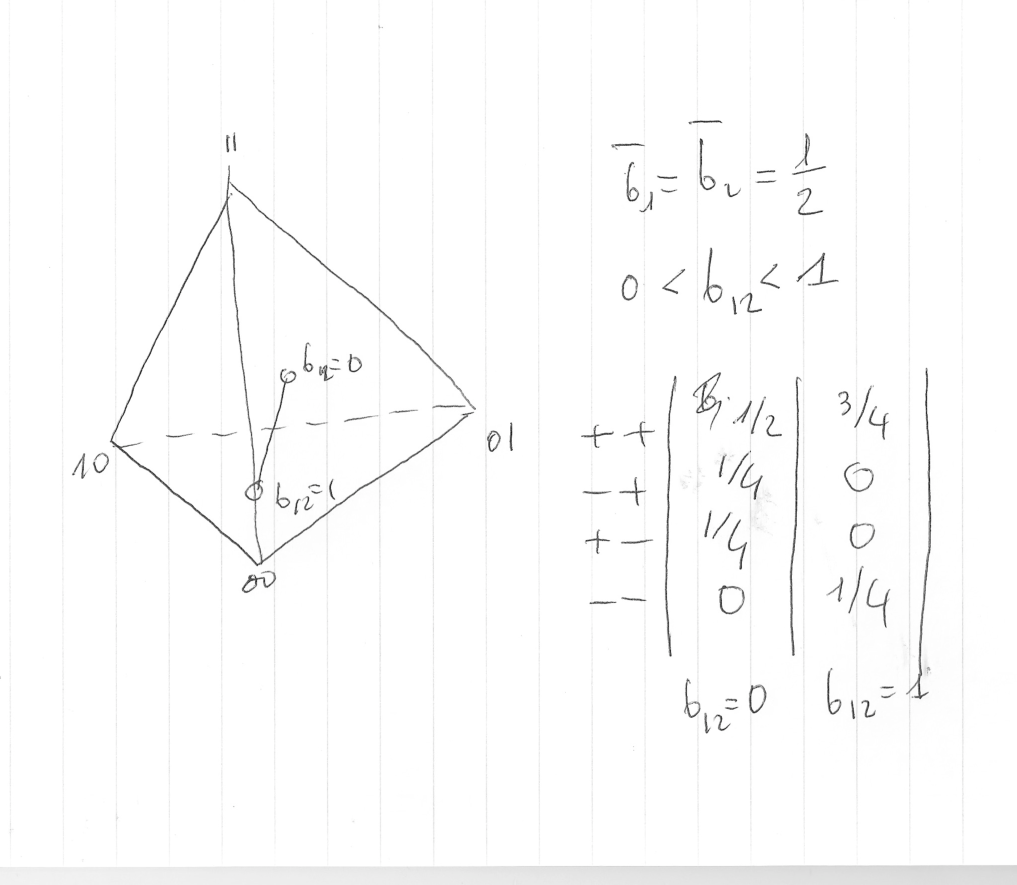
\includegraphics[width=.4\textwidth]{plan2x2.pdf}
    \caption{Plan on binary sample space}
    \label{fig:1}
  \end{figure}
%
We start with the case $n_1=n_2=2$. Let $\Omega_1=\Omega_2=\set{+,-}$, $\Omega=\set{++,+-,-+,--}$ Any function on $\Omega$ has the pseudo-Boolean form $f(x,y)=a_0+a_1 x + a_2 y + a_{12} xy$. In particular a probability has the form $\gamma(x,y) = \frac14(1+b_1x+b_2y+b_{12}xy)$ with $\gamma_1(x) = X_{\#}\gamma (x)= \frac12(1+b_1x)$, $\gamma_2(y) = Y_\# \gamma(y) = \frac12(1+b_2y)$. Given $\bar b_1, \bar b_2 \in ]-1,+1[$ to fix the margins, the plan is given by the 1 parameter family 
%
  \begin{equation*}
    \gamma(x,y) = \frac14(1+\bar b_1x+\bar b_2y+b_{12}xy), \quad -1 + \avalof{\bar b_1+\bar b_2} < b_{12} < 1 - \avalof{\bar b_1 - \bar b_2} \ .
  \end{equation*}
\end{exercise}

\subsection{Gradient flow}

\begin{proposition}Let be given a cost function $c \colon \Omega_1 \times \Omega_2 \to \reals$ and define the expected cost function $C \colon \SimO \ni \gamma \mapsto \expectat \gamma c$. Then the function $C$ restricted to the open plan $\Gamma^\circ(\mu_1,\mu_2)$ has statistical gradient
%
\begin{equation*}
 \grad_{\Gamma(\mu_1,\mu_2)} W \colon \gamma \mapsto w - \expectat \gamma w - w_{1,\gamma} - w_{2,\gamma} \in S_\gamma\Gamma(\mu_1,\mu_2) = (S_\gamma \oSimO)_{12} \ . 
\end{equation*}

It follows that the gradient flow of $W$ is
%
\begin{equation*}
  D\gamma(t) = - \left(w - \expectat \gamma w - w_{1,\gamma} - w_{2,\gamma}\right) \ .
\end{equation*}

Any solution $t \mapsto \gamma(t)$ of the gradient flow converges to a measure $\gamma* = \lim_{t \to \infty} \gamma(t) \in \SimO$ such that $\expectat {\gamma^*} w$ is the \emph{Gini dissimilarity} or \emph{Wasserstein distance} between $\mu_1$ and $\mu_2$,
%
\begin{equation*}
  \expectat {\gamma*} w = \min \setof{\expectat \gamma w}{ \gamma \in \Gamma(\mu_1,\mu_2)} \ .
\end{equation*}
%
 Moreover, the extension of the gradient to $\SimO$ is zero at $\gamma^*$, namely
%
\begin{equation*}
  w = \expectat {\gamma^*} w + w_{1,\gamma^*} + w_{2,\gamma^*}
\end{equation*}
%
on $\suppof{\gamma^*}$.
\end{proposition}

\begin{proof}
  
\end{proof}

\subsection{Kantorovich}

\bibliography{discrete-wasserstein}

\end{document}

